As introduced in \autoref{sec:intro-external-nondet}, the environment might
affect the transmission of messages, so called external nondeterminism.  The
tester should take the environment into account when validating its
observations.

This section explains how to address external nondeterminism by specifying the
environment, with the networked server example.  \autoref{sec:net-tcp} defines a
model for concurrent TCP connections.  \autoref{sec:net-compose} then composes
the network model with the server specification, yielding a tester-side
specification that defines the space of valid observations.

\subsection{Modelling the network}
\label{sec:net-tcp}
When testing servers over the network, request and response packets may be
indefinitely delayed.  As a result, messages from one end might arrive at the
other end in a different order from that they were sent.

The space of network reorderings can be modelled by a {\em network model}, a
conceptual program for the ``network wire''.  The wire can be viewed as a
buffer, which absorbs packets and later emits them:
\begin{coq}
  Variant netE: Type -> Type := (* network event type *)
    Emit  : packet -> netE unit
  | Absorb: netE packet.
\end{coq}

After absorbing a packet, the wire may emit it immediately or after
absorbing/emitting other packets.  Such choices are modelled by nondeterministic
\ilc{Or} branches:
\begin{coq}
  Variant nondetE: Type -> Type := (* nondeterministic branch *)
    Or: nondetE bool.

  Definition or {E R} `{nondetE -< E} (x y: itree E R) : itree E R :=
    b <- trigger Or;;
    if b then x else y.
\end{coq}

Here \ilc{(or x y)} creates a nondeterministic program that may behave as either
\ilc x or \ilc y.  The \ilc{nondetE} here is a special case of \ilc{choiceE}
defined in \autoref{sec:itree-lang} with boolean space of choices, but they'll
be handled differently during test derivation.  The type signature \ilc{\{E R\}
  `\{nondetE -< E\}} says the \ilc{(or)} combinator can apply to ITrees whose
event \ilc E is a super-event of \ilc{nondetE}, and with arbitrary return type
\ilc R.  For example, arguments \ilc x and \ilc y can be of type \ilc{(itree
  (netE +' nondetE) void)}.

For example, the network model for concurrent TCP connections is defined in
\autoref{fig:tcp-model}.  The model captures TCP's feature of maintaining the
order within each connection, but packets in different connections might be
reordered arbitrarily.  When the wire chooses a packet to send, the candidate
must be the oldest in its connection.

\begin{figure}
\begin{coq}
Fixpoint pick_one (l: list packet) : itree nondetE (option packet) :=
  if l is p::l'
  then or (Ret (Some p)) (pick_one l')
  else ret None.

Definition oldest_in_each_conn : list packet -> list packet := ...
(* filter the oldest packet in each connection *)

CoFixpoint tcp (buffer: list packet) : itree (netE +' nondetE) void :=
  let absorb := pkt <- trigger Absorb;;
                tcp (buffer ++ [pkt])      in
  let emit p := trigger (Emit p);;
                tcp (remove pkt buffer)    in
  let pkts   := oldest_in_each_conn buffer in
  opkt <- pick_one pkts;;
  if opkt is Some pkt
  then emit pkt
  else absorb.
\end{coq}
\caption[Network model for concurrent TCP connections]{Network model for
  concurrent TCP connections.  The model is an infinite program iterating over a
  \ilc{buffer} of all packets en route.  In each iteration, the model either
  \ilc{absorb}s or \ilc{emit}s some packet, depending on the current
  \ilc{buffer} state and the choice made in \ilc{pick_one}.  Any absorbed packet
  is appended to the end of buffer.  When emitting a packet, the model may
  choose a connection and send the oldest packet in it.}
\label{fig:tcp-model}
\end{figure}

Notice the \ilc{pick_one} function, which might return (i) \ilc{Some p} or (ii)
\ilc{None}.  \lys{Should I explain what is option type?}  The network model then
(i) emits packet \ilc p or (ii) absorbs a packet into \ilc{buffer}.

\begin{itemize}
\item When the given list \ilc{pkts} is empty, \ilc{pick_one} always returns
  \ilc{None}, becuase the wire has no packet in the \ilc{buffer}, and must
  absorb some packet before emitting anything.
\item Given a non-empty linked list \ilc{(p::l')}, with \ilc p as head and
  \ilc{l'} as tail, \ilc{pick_one} might return \ilc{(Some p)}, meaning the wire
  can emit that packet; or it might return \ilc{None}, meaning the wire can
  still absorb packets into the buffer.
\end{itemize}

Such network model reflects the TCP environment, where messages are never lost
but might be indefinitely delayed.  In the next subsection, I'll demonstrate how
to compose the server and network models into a client-side observation model.

\subsection{Network composition}
\label{sec:net-compose}

The network connects the server on one end to the clients on other ends.  When
one end sends some message, the network model absorbs it and later emits it to
the destination.

To {\em compose} a server model with a network model is to pair the server's
\ilc{Send} and \ilc{Recv} events with the network's \ilc{Absorb} and \ilc{Emit}
events.  Since the network model is nondeterministic, it might not be ready to
absorb packets sent by the server.  The network might also emit a packet before
the server is ready to receive it.

\begin{figure}
  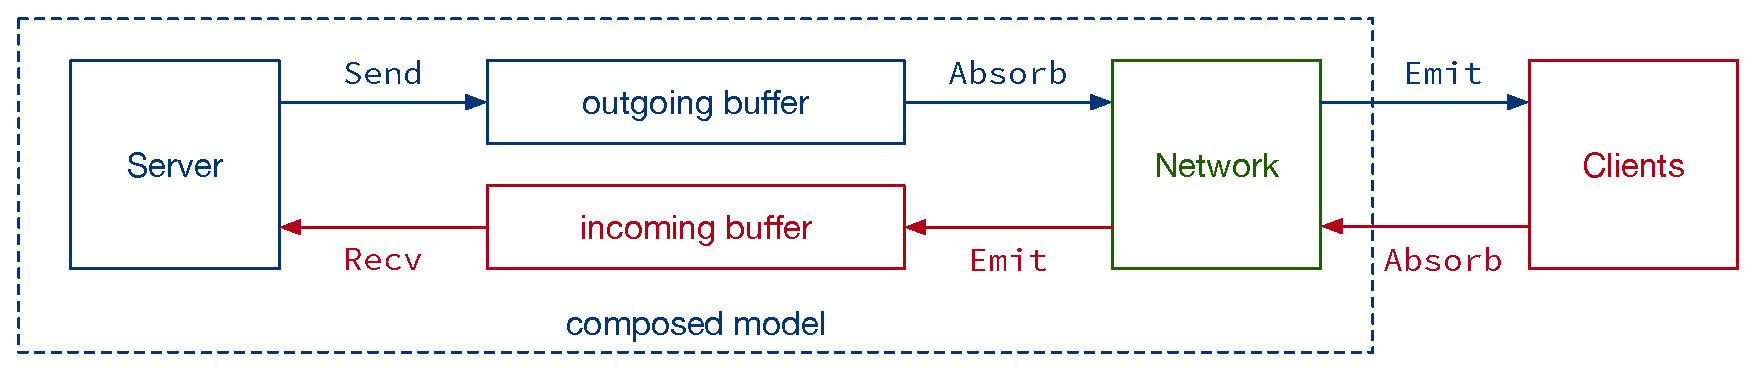
\includegraphics[width=\textwidth]{figures/net-compose}
  \caption{Network composition architecture}
  \label{fig:net-compose}
\end{figure}

To handle the asynchronicity among the server and network events, I insert
message buffers between them.  As shown in \autoref{fig:net-compose}, the {\em
  incoming buffer} stores the packets emitted by the network but not yet
consumed by the server's \ilc{Recv} events, and the {\em outgoing buffer} stores
the packets sent by the server but not yet absorbed by the network.

\begin{figure}
\begin{lstlisting}[style=customcoq,numbers=left,escapechar=\%]
CoFixpoint compose {E} (srv: itree (qaE +' E) void)   (* server  model *)
           (net  : itree (netE +' nondetE) void)      (* network model *)
           (bi bo: list packet)       (* incoming and outgoing buffers *)
           : itree (netE +' nondetE +' E) void :=
  let step_net :=%\label{line:step-net-def}%
    match net with
    | Impure (Absorb|) knet =>
      if bo is pkt::bo'
      then compose srv (knet pkt) bi bo'%\label{line:net-absorb}%
      else pkt <- trigger Absorb;;%\label{line:client-send}%
           compose srv (knet pkt) bi bo
    | Impure (Emit pkt|) knet =>
      if toServer pkt
      then compose srv (knet tt) (bi++[pkt]) bo%\label{line:srv-incoming}%
      else trigger (Emit pkt);;%\label{line:net-emit}%
           compose srv (knet tt) bi bo
    | Impure (|Or) knet => b <- trigger Or;;
                        compose srv (knet b) bi bo
    | Pure vd => match vd in void with end
    end
  in
  match srv with
  | Impure (Recv|) ksrv =>
    if bi is pkt::bi'
    then compose (ksrv pkt) net bi' bo%\label{line:srv-consume}%
    else step_net%\label{line:step-net}%
  | Impure (Send pkt|) ksrv =>%\label{line:srv-send}%
    compose (ksrv tt) net bi (bo++[pkt])
  | Impure (|e) ksrv =>        (* other events performed by the server *)
    r <- trigger e;; compose (ksrv r) net bi bo
  | Pure vd => match vd in void with end
  end.
\end{lstlisting}
\caption[Network composition algorithm]{Network composition algorithm.  When the
  server wants to send a packet in \autoref{line:srv-send}, the packet is
  appended to the outgoing buffer until absorbed by the network in
  \autoref{line:net-absorb}, and eventually emitted to the client in
  \autoref{line:net-emit}.  Conversely, packets sent by clients are absorbed by
  the network in \autoref{line:client-send}, emitted to the server's incoming
  buffer in \autoref{line:srv-incoming}, until the server consumes it in
  \autoref{line:srv-consume}.}
\label{fig:net-compose-code}
\end{figure}

The server and the clients are the opposite ends of the network.  Each packet
has routing fields that indicate its source and destination.  When the network
emits a packet, we need to determine whether the packet is emitted to the
server's incoming buffer or to the clients, by inspecting its destination:
\begin{coq}
  Record packet := {
    source      : connection;
    destination : connection;
    payload     : data
  }.

  Definition toServer (p: packet) : bool :=
    if p.(destination) is server_conn then true else false.
\end{coq}

Now we can define the composition algorithm formally, as shown in
\autoref{fig:net-compose-code}.  In this example, we reuse the \ilc{qaE}
definition in \autoref{sec:itree-lang}, and let the \ilc Q and \ilc A both be
the \ilc{packet} type.  The composed ITree takes the server and network models
as parameters, and makes steps in the two ITrees in certain order.

The composed model exhibits to the client three kinds of events: (i) Network
operations (\ilc{netE}) where packets are emitted to or absorbed from clients,
(ii) Nondetermistic branches (\ilc{nondetE}) made by the network model, and
(iii) Other events \ilc{\{E\}} performed by the server model {\it e.g.} internal
choices (\ilc{choiceE}) in \autoref{sec:itree-lang}.

Notice that this algorithm schedules the server at a higher priority than the
network model.  The composed model only steps into the network model when the
server is starved in \autoref{line:step-net}, by calling the \ilc{step_net}
process defined in \autoref{line:step-net-def}.  Such design is to avoid
divergence of the derived tester program, which I'll further explain in
\autoref{sec:spec-to-test}.

So far I've shown how to specify systems that exhibit external nondeterminism.
By specifying the environment and composing it with the implementation-side
specification, we can describe the space of valid observations.  The rest of
this chapter will show how to derive tester programs from the observer-side
specification.
